% !TeX spellcheck = cs_CZ
%{\tikzset{external/prefix={tikz/FYZII/}}
% \tikzset{external/figure name/.add={ch36_}{}}
%---------------------------------------------------------------------------------------------------
% file fey2ch36.tex
%---------------------------------------------------------------------------------------------------
%=========================== Kapitola Feromagnetizmus ==============================================
\setchaptertoc
\chapter{Feromagnetizmus}\label{fyz:IIchapXXXVI}

  \section{Magnetizační proudy}\label{fyz:IIchapXXXVIsecI}
  \section{Pole H}\label{fyz:IIchapXXXVIsecII}
  \section{Magnetizační křivka}\label{fyz:IIchapXXXVIsecIII}
  \section{Indukčnost ocelových jader}\label{fyz:IIchapXXXVIsecIV}
  \section{Elektromagnety}\label{fyz:IIchapXXXVIsecV}
  \section{Spontánní magnetizace}\label{fyz:IIchapXXXVIsecVI}
  \section{Příklady a cvičení}\label{fyz:IIchapXXXVIsecVII}

    \begin{figure}[ht!] %\ref{fyz:fig831}
      \centering
      \subcaptionbox{\label{fyz:fig831a}}{\luafigure[0.9]{fyz_fig831a.pdf}}               \newline
      \subcaptionbox{\label{fyz:fig831b}}{\luafigure[0.9]{fyz_fig831b.pdf}}               \newline
      \subcaptionbox{\label{fyz:fig831c}}{\luafigure[0.9]{fyz_fig831c.pdf}}
      \caption{
               (\cite[s.~748]{Feynman02})}
      \label{fyz:fig831}
    \end{figure}

    \begin{figure}[ht!] %\ref{fyz:fig832}
      \centering
      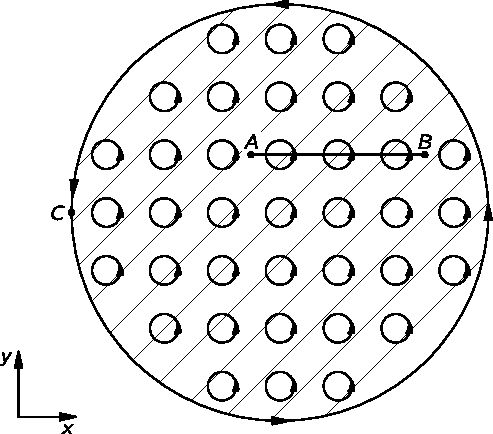
\includegraphics[width=0.7\linewidth]{fyz_fig832.pdf}
      \caption{
               (\cite[s.~707]{Feynman02})}
      \label{fyz:fig832}
    \end{figure}
    
    \begin{figure}[ht!] %\ref{fyz:fig833}
      \centering
      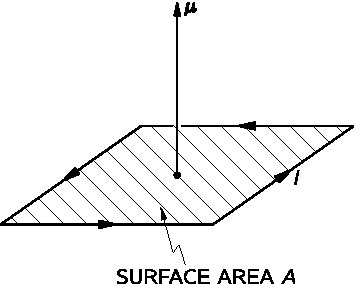
\includegraphics[width=0.7\linewidth]{fyz_fig833.pdf}
      \caption{
               (\cite[s.~707]{Feynman02})}
      \label{fyz:fig833}
    \end{figure}
    
    \begin{figure}[ht!] %\ref{fyz:fig834}
      \centering
      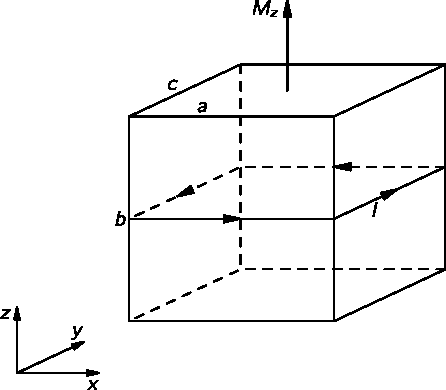
\includegraphics[width=0.7\linewidth]{fyz_fig834.pdf}
      \caption{
               (\cite[s.~707]{Feynman02})}
      \label{fyz:fig834}
    \end{figure}
    
    \begin{figure}[ht!] %\ref{fyz:fig835}
      \centering
      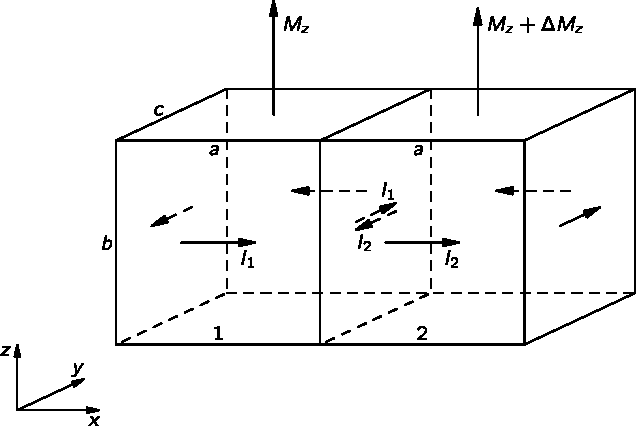
\includegraphics[width=0.7\linewidth]{fyz_fig835.pdf}
      \caption{
               (\cite[s.~707]{Feynman02})}
      \label{fyz:fig835}
    \end{figure}
    
    \begin{figure}[ht!] %\ref{fyz:fig836}
      \centering
      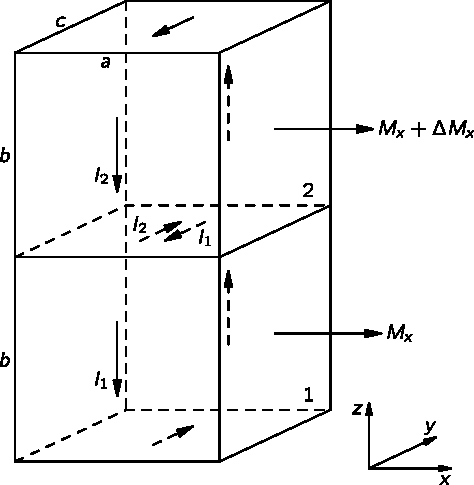
\includegraphics[width=0.7\linewidth]{fyz_fig836.pdf}
      \caption{
               (\cite[s.~707]{Feynman02})}
      \label{fyz:fig836}
    \end{figure}

    \begin{figure}[ht!] %\ref{fyz:fig837}
      \centering
      \subcaptionbox{\label{fyz:fig837a}}{\luafigure[0.9]{fyz_fig837a.pdf}}               \newline
      \subcaptionbox{\label{fyz:fig837b}}{\luafigure[0.9]{fyz_fig837b.pdf}}
      \caption{
               (\cite[s.~748]{Feynman02})}
      \label{fyz:fig837}
    \end{figure}

    \begin{figure}[ht!] %\ref{fyz:fig838}
      \centering
      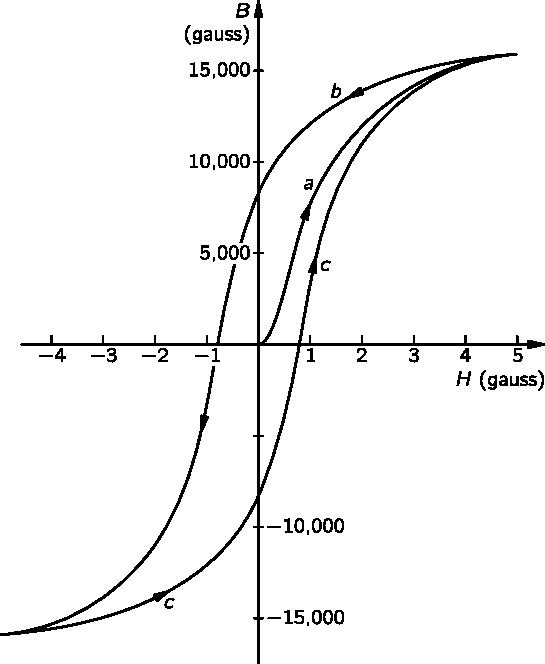
\includegraphics[width=0.7\linewidth]{fyz_fig838.pdf}
      \caption{
               (\cite[s.~707]{Feynman02})}
      \label{fyz:fig838}
    \end{figure}

    \begin{figure}[ht!] %\ref{fyz:fig839}
      \centering
      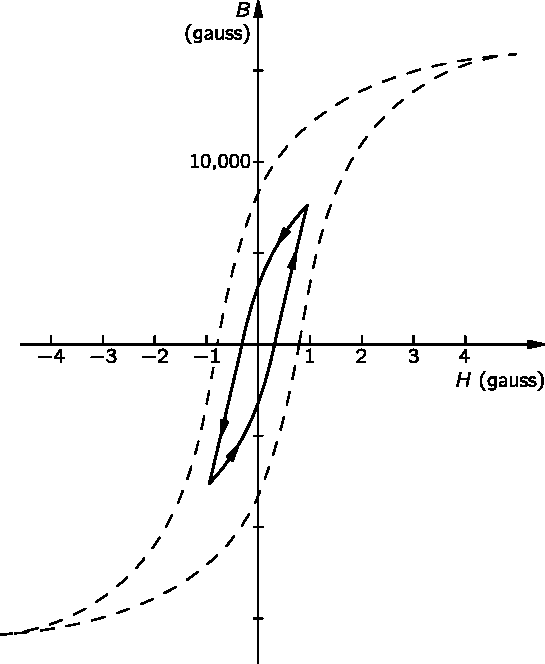
\includegraphics[width=0.7\linewidth]{fyz_fig839.pdf}
      \caption{
               (\cite[s.~707]{Feynman02})}
      \label{fyz:fig839}
    \end{figure}

    \begin{figure}[ht!] %\ref{fyz:fig840}
      \centering
      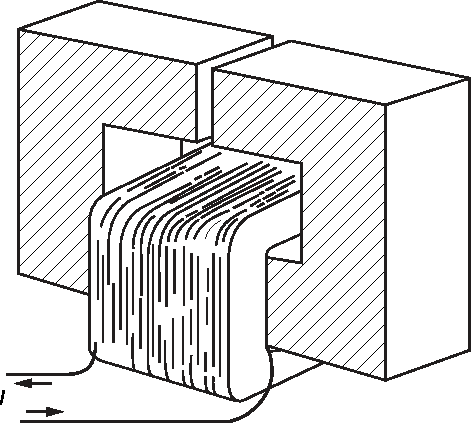
\includegraphics[width=0.7\linewidth]{fyz_fig840.pdf}
      \caption{
               (\cite[s.~707]{Feynman02})}
      \label{fyz:fig840}
    \end{figure}
    
    \begin{figure}[ht!] %\ref{fyz:fig841}
      \centering
      \subcaptionbox{\label{fyz:fig841a}}{\luafigure[0.9]{fyz_fig841a.pdf}}               \newline
      \subcaptionbox{\label{fyz:fig841b}}{\luafigure[0.9]{fyz_fig841b.pdf}}
      \caption{
               (\cite[s.~748]{Feynman02})}
      \label{fyz:fig841}
    \end{figure}

    \begin{figure}[ht!] %\ref{fyz:fig842}
      \centering
      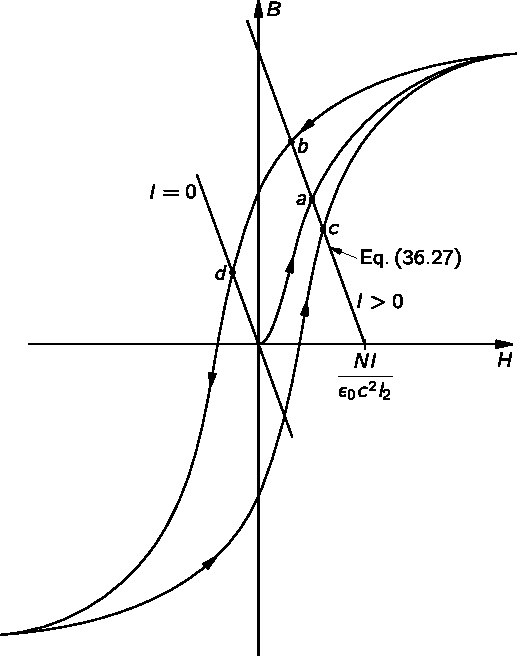
\includegraphics[width=0.7\linewidth]{fyz_fig842.pdf}
      \caption{
               (\cite[s.~707]{Feynman02})}
      \label{fyz:fig842}
    \end{figure}

    \begin{figure}[ht!] %\ref{fyz:fig843}
      \centering
      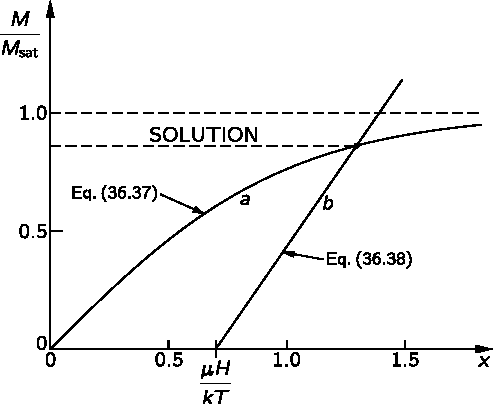
\includegraphics[width=0.7\linewidth]{fyz_fig843.pdf}
      \caption{
               (\cite[s.~707]{Feynman02})}
      \label{fyz:fig843}
    \end{figure}

    \begin{figure}[ht!] %\ref{fyz:fig844}
      \centering
      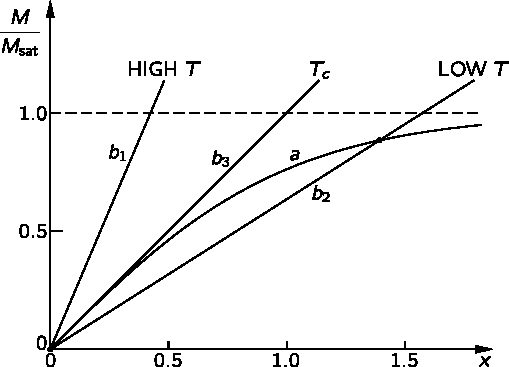
\includegraphics[width=0.7\linewidth]{fyz_fig844.pdf}
      \caption{
               (\cite[s.~707]{Feynman02})}
      \label{fyz:fig844}
    \end{figure}

    \begin{figure}[ht!] %\ref{fyz:fig845}
      \centering
      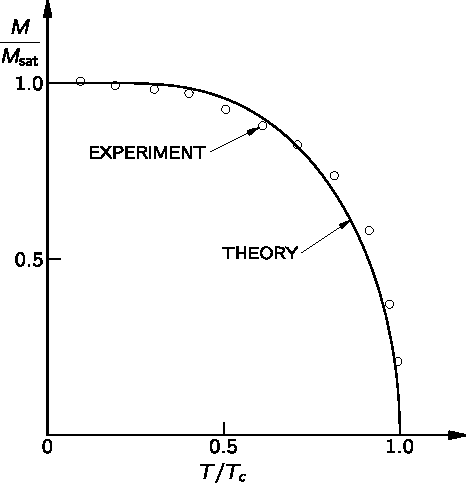
\includegraphics[width=0.7\linewidth]{fyz_fig845.pdf}
      \caption{
               (\cite[s.~707]{Feynman02})}
      \label{fyz:fig845}
    \end{figure}

    \todo[inline]{Kapitola fey1ch36 je zcela prázdná, pouze obrázky}  
%} %tikzset
%---------------------------------------------------------------------------------------------------